\documentclass[11pt]{article}
\usepackage{amsmath, amssymb, bm}
\usepackage[colorlinks=true,linkcolor=blue,citecolor=blue,urlcolor=blue]{hyperref}
\usepackage{url}
\usepackage{geometry}
\usepackage{graphicx}
\usepackage{float}
\usepackage{subcaption}
\usepackage{listings}
\usepackage{xcolor}
\geometry{margin=1in}

% Code listing setup
\lstset{
    basicstyle=\ttfamily\footnotesize,
    backgroundcolor=\color{gray!10},
    keywordstyle=\color{blue},
    commentstyle=\color{green!40!black},
    stringstyle=\color{red},
    numbers=left,
    numberstyle=\tiny,
    stepnumber=1,
    numbersep=5pt,
    frame=single,
    breaklines=true,
    breakatwhitespace=true,
    showstringspaces=false
}

\title{Hexapod Kinematics with Geometric Algebra:\\A Comprehensive Tutorial and Implementation Guide}
\author{Prepared for Bj\o rn Remseth}
\date{\today}

\begin{document}
\maketitle

\tableofcontents
\newpage

\section{Introduction}

This document serves as both a comprehensive tutorial on geometric algebra applications in robotics and a practical implementation guide for the \texttt{goik-ga} library. We focus specifically on hexapod leg kinematics as a compelling case study that demonstrates the power and elegance of geometric algebra (GA) methods compared to traditional matrix-based approaches.

\noindent\textbf{Acknowledgment:} This work is strongly inspired by and builds upon the excellent foundation provided by Hans Jørgen Grimstad's \texttt{goik} package~\footnote{\url{https://github.com/hansj66/goik/tree/main/goik}}, which pioneered practical hexapod kinematics implementations in Go. Our contribution refactors this work to use geometric algebra primitives for improved mathematical clarity and computational efficiency.

\subsection{Why This Tutorial Matters}

Traditional robotics often relies on rotation matrices, Euler angles, and homogeneous transformations. While functional, these approaches suffer from:
\begin{itemize}
    \item \textbf{Gimbal lock:} Euler angles become singular at certain configurations
    \item \textbf{Computational overhead:} Matrix multiplications are expensive and accumulate numerical errors
    \item \textbf{Frame bookkeeping complexity:} Managing coordinate frame transformations becomes unwieldy
    \item \textbf{Non-intuitive composition:} Multiple transformations require careful ordering and mental overhead
\end{itemize}

Geometric algebra, particularly through \emph{motors} (the GA equivalent of dual quaternions), provides a unified, efficient, and mathematically elegant alternative that addresses all these issues.

\section{Geometric Algebra Foundations}

Before diving into hexapod kinematics, we establish the mathematical foundations that make our approach both powerful and intuitive.

\subsection{What is Geometric Algebra?}

Geometric algebra extends vector algebra to include oriented areas (bivectors), volumes (trivectors), and higher-dimensional entities. The key insight is that geometric products naturally encode both the magnitude and orientation of geometric transformations.

For 3D space, we work in Clifford algebra $Cl(3,0,1)$ with basis elements:
\begin{align}
    &\text{Scalars: } 1\\
    &\text{Vectors: } \mathbf{e}_1, \mathbf{e}_2, \mathbf{e}_3\\
    &\text{Bivectors: } \mathbf{e}_{12}, \mathbf{e}_{23}, \mathbf{e}_{31}\\
    &\text{Trivector: } \mathbf{e}_{123}\\
    &\text{Pseudoscalar: } \mathbf{e}_0
\end{align}

\subsection{Projective vs. Conformal Geometric Algebra}

Our implementation supports two complementary approaches:

\paragraph{Projective Geometric Algebra (PGA).}
PGA represents rigid motions (rotations + translations) as \emph{motors}~\cite{gunn2011pga}, which you can view as the geometric-algebraic analog of dual quaternions. The key advantages:
\begin{itemize}
    \item Unified representation of rotations and translations
    \item Associative composition: $(M_1 \cdot M_2) \cdot M_3 = M_1 \cdot (M_2 \cdot M_3)$
    \item Natural interpolation between poses
    \item Efficient sandwich product for point transformation: $X' = M X \tilde{M}$
\end{itemize}

\paragraph{Conformal Geometric Algebra (CGA).}
CGA encodes points as null vectors and treats planes, lines, circles, and spheres as native geometric objects~\cite{dorst2009gacs}. Benefits include:
\begin{itemize}
    \item Translations become rotations in higher-dimensional space
    \item Natural meet/join operations for intersections and constraints
    \item Direct computation of distances and projections
    \item Elegant handling of degenerate cases
\end{itemize}

Our current implementation focuses on PGA for production use, with CGA as a parallel API for future enhancement.

\section{Mathematical Representation Details}

\subsection{Motors as Dual Quaternions}

In our PGA implementation, motors are represented as dual quaternions $(r + \varepsilon d)$ where:
\begin{itemize}
    \item $r$ is a unit quaternion representing rotation
    \item $d$ is the dual part encoding translation  
    \item $\varepsilon$ is the dual unit with $\varepsilon^2 = 0$
\end{itemize}

Given axis-angle rotation $(\mathbf{\hat{u}}, \theta)$ and translation $\mathbf{t}$:
\begin{align}
r &= \cos \frac{\theta}{2} + \sin \frac{\theta}{2} \, (\hat{u}_x \mathbf{i} + \hat{u}_y \mathbf{j} + \hat{u}_z \mathbf{k})\\
d &= \frac{1}{2} \, \mathbf{t}\, r
\end{align}

Composition follows dual quaternion multiplication:
\[(r_1, d_1)(r_2, d_2) = (r_1 r_2,\; r_1 d_2 + d_1 r_2)\]

Point transformation uses the sandwich product:
\[\mathbf{p}' = r\,\mathbf{p}\,r^* + 2\,\mathrm{vec}(d\,r^*)\]

This matches the PGA motor action for SE(3) rigid body motions.

\begin{figure}[H]
    \centering
    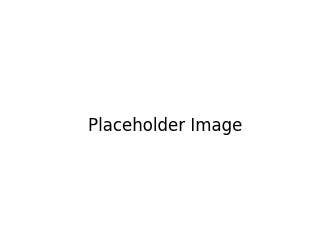
\includegraphics[width=0.8\textwidth]{illustrations/motor_composition.png}
    \caption{Motor composition workflow showing the associative nature of geometric transformations. Each motor represents a screw motion (combined rotation and translation), and their composition naturally represents the complete kinematic chain.}
    \label{fig:motor_composition}
\end{figure}

\section{Hexapod Leg Kinematics: Case Study}

Now we apply these concepts to a concrete robotics problem: computing the forward and inverse kinematics of a 3-degree-of-freedom hexapod leg.

\subsection{Leg Structure and Configuration}

Our hexapod leg consists of three joints in series:
\begin{enumerate}
    \item \textbf{Hip Joint (J1):} Yaw rotation about Z-axis, range typically $\pm 45^\circ$
    \item \textbf{Thigh Joint (J2):} Pitch rotation about Y-axis, forward/backward swing
    \item \textbf{Knee Joint (J3):} Pitch rotation about Y-axis, leg extension/flexion
\end{enumerate}

The leg geometry parameters are:
\begin{itemize}
    \item $l_1 = 0.05$ m: Hip offset (lateral displacement to thigh joint)
    \item $l_2 = 0.20$ m: Thigh length
    \item $l_3 = 0.20$ m: Shank length  
\end{itemize}

\begin{figure}[H]
    \centering
    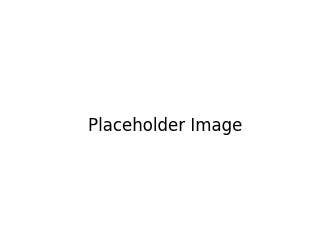
\includegraphics[width=0.7\textwidth]{illustrations/hexapod_leg_structure.png}
    \caption{Hexapod leg structure showing the three joints and their motion axes. Each joint contributes a motor to the overall kinematic chain.}
    \label{fig:leg_structure}
\end{figure}

\subsection{Coordinate Frame Relationships}

The kinematic chain establishes a sequence of coordinate frame transformations from the robot base to the toe. Each transformation is represented by a motor that encodes both the joint rotation and any necessary translation.

\begin{figure}[H]
    \centering
    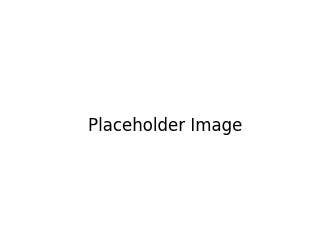
\includegraphics[width=0.8\textwidth]{illustrations/coordinate_frames.png}
    \caption{Coordinate frame relationships in the hexapod leg. Each frame transformation is represented by a geometric algebra motor, eliminating the need for separate rotation matrices and translation vectors.}
    \label{fig:coordinate_frames}
\end{figure}

The coordinate system conventions are:
\begin{itemize}
    \item \textbf{X-axis:} Forward direction (leg extension)
    \item \textbf{Y-axis:} Lateral direction (leg abduction)  
    \item \textbf{Z-axis:} Vertical direction (leg lift)
\end{itemize}

\section{Forward Kinematics Implementation}

\subsection{Motor Chain Construction}

Forward kinematics involves constructing a chain of motors and applying them to compute the toe position. Each joint contributes a screw motor that combines rotation about the joint axis with any necessary translation.

\begin{lstlisting}[language=Go, caption=Forward kinematics implementation in Go]
func main() {
    // Physical parameters
    l1 := 0.05  // hip offset to thigh (m)
    l2 := 0.20  // thigh length  
    l3 := 0.20  // shank length

    // Joint centers
    hip := pga.V(0, 0, 0)
    thighJ := hip.Add(pga.V(l1, 0, 0))
    kneeJ := thighJ.Add(pga.V(l2, 0, 0))

    // Joint axes
    z := pga.V(0, 0, 1)  // Hip yaw axis
    y := pga.V(0, 1, 0)  // Pitch axes

    // Joint angles (example configuration)
    theta1 := 20 * math.Pi / 180   // Hip yaw
    theta2 := -10 * math.Pi / 180  // Thigh pitch  
    theta3 := 30 * math.Pi / 180   // Knee pitch

    // Build motor chain
    M := pga.Identity().
        Mul(pga.Screw(hip, z, theta1, 0)).       // Hip yaw
        Mul(pga.Screw(thighJ, y, theta2, 0)).    // Thigh pitch
        Mul(pga.Screw(kneeJ, y, theta3, 0)).     // Knee pitch  
        Mul(pga.Translator(pga.V(l3, 0, 0)))     // Toe offset

    // Compute toe position
    toe0 := pga.V(0, 0, 0)  // Initial toe position
    toe := M.ActPoint(toe0)  // Final toe position
}
\end{lstlisting}

\subsection{Geometric Interpretation}

The beauty of the motor approach is that each transformation has a clear geometric interpretation:

\begin{align}
\mathbf{P}_{\text{toe}} &= M_{\text{total}} \cdot \mathbf{P}_0 \cdot \tilde{M}_{\text{total}}\\
\text{where } M_{\text{total}} &= M_{\text{identity}} \cdot M_{\text{hip}} \cdot M_{\text{thigh}} \cdot M_{\text{knee}} \cdot M_{\text{translation}}
\end{align}

Each motor $M_i$ represents a screw motion:
\[M_i = \text{Screw}(\mathbf{center}, \mathbf{axis}, \theta_i, \text{pitch})\]

For pure rotations, the pitch is zero. The final translation motor moves from the knee joint to the toe along the shank.

\begin{figure}[H]
    \centering
    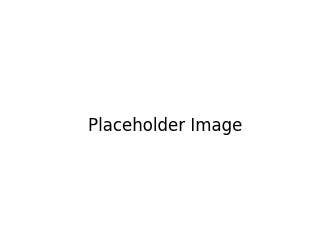
\includegraphics[width=\textwidth]{illustrations/leg_configuration-py.png}
    \caption{3D visualization of the hexapod leg configuration showing joint positions, link lengths, and the resulting toe position. The coordinate frames and joint angles are clearly visible, demonstrating the geometric relationships in the kinematic chain.}
    \label{fig:leg_config}
\end{figure}

\section{Velocity Analysis and Jacobians}

For motion control and trajectory planning, we need to understand how joint velocities map to end-effector velocities. This relationship is captured by the Jacobian matrix.

\subsection{Jacobian Column Computation}

Each column of the Jacobian represents the instantaneous linear velocity of the toe when the corresponding joint rotates at unit angular velocity. For a revolute joint, this is computed using the cross product:

\[\mathbf{J}_i = \hat{\mathbf{u}}_i \times (\mathbf{p}_{\text{toe}} - \mathbf{c}_i)\]

where:
\begin{itemize}
    \item $\hat{\mathbf{u}}_i$ is the unit axis of joint $i$
    \item $\mathbf{c}_i$ is the center point of joint $i$  
    \item $\mathbf{p}_{\text{toe}}$ is the current toe position
\end{itemize}

\begin{lstlisting}[language=Go, caption=Jacobian computation for velocity analysis]
// Jacobian columns at current pose (linear velocity for each joint)
J1 := pga.RevoluteColumn(hip, z, toe)      // Hip yaw contribution
J2 := pga.RevoluteColumn(thighJ, y, toe)   // Thigh pitch contribution  
J3 := pga.RevoluteColumn(kneeJ, y, toe)    // Knee pitch contribution

// Build complete Jacobian matrix: J = [J1 J2 J3]
// Joint velocities map to toe velocity: v_toe = J * [theta_dot1 theta_dot2 theta_dot3]^T
\end{lstlisting}

\subsection{Physical Interpretation of Jacobian Columns}

Each Jacobian column has a clear physical meaning:

\begin{itemize}
    \item \textbf{J1 (Hip):} Creates circular motion in the XY plane around the Z-axis
    \item \textbf{J2 (Thigh):} Affects primarily X and Z components, swinging the leg forward/backward
    \item \textbf{J3 (Knee):} Contributes to leg extension, affecting X and Z components
\end{itemize}

\begin{figure}[H]
    \centering
    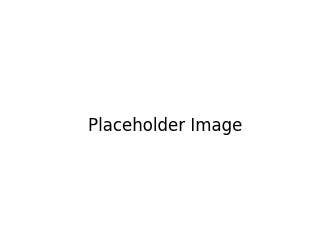
\includegraphics[width=\textwidth]{illustrations/jacobian_visualization-py.png}
    \caption{Visualization of Jacobian columns showing the instantaneous velocity directions for each joint. The 3D plot shows how each joint contributes to toe motion, while the 2D projections illustrate the velocity components in different planes.}
    \label{fig:jacobian_viz}
\end{figure}

\section{Inverse Kinematics Strategies}

While forward kinematics is straightforward with motors, inverse kinematics requires more sophisticated approaches. We present both analytical and numerical methods.

\subsection{Analytical Inverse Kinematics}

For many hexapod leg configurations, analytical solutions exist by exploiting the geometric structure:

\paragraph{Hip Yaw Angle.} The hip yaw angle can be computed from the desired toe position projection:
\[\theta_1 = \text{atan2}(y_{\text{toe}}, x_{\text{toe}})\]

\paragraph{Planar Two-Link Problem.} After accounting for hip yaw, the thigh-knee pair forms a planar two-link mechanism. Using the cosine law on the triangle formed by hip, knee, and toe:
\begin{align}
d &= \sqrt{x_{\text{toe}}^2 + z_{\text{toe}}^2}\\
\cos(\theta_3) &= \frac{d^2 - l_2^2 - l_3^2}{2 l_2 l_3}\\
\theta_2 &= \text{atan2}(z_{\text{toe}}, x_{\text{toe}}) - \text{atan2}(l_3 \sin(\theta_3), l_2 + l_3 \cos(\theta_3))
\end{align}

\subsection{Numerical Inverse Kinematics}

For more complex configurations or constraints, numerical methods using the Jacobian provide a general solution:

\[\Delta \boldsymbol{\theta} = J^{\dagger} (\mathbf{x}^* - \mathbf{x})\]

where $J^{\dagger}$ is the pseudoinverse of the Jacobian, providing damped least-squares solutions that handle singularities gracefully.

\section{Performance and Robustness Analysis}

\subsection{Computational Complexity}

The motor-based approach offers significant computational advantages:

\begin{itemize}
    \item \textbf{Forward kinematics:} $O(n)$ motor multiplications vs. $O(n^3)$ matrix operations
    \item \textbf{Memory efficiency:} 8 floats per motor vs. 16 floats per homogeneous matrix
    \item \textbf{Numerical stability:} Quaternion normalization is cheaper and more stable than matrix orthogonalization
\end{itemize}

\subsection{Robustness Considerations}

Geometric algebra methods are inherently more robust:

\begin{itemize}
    \item \textbf{No gimbal lock:} Motors avoid the singularities of Euler angles
    \item \textbf{Smooth interpolation:} Motor SLERP provides natural pose interpolation
    \item \textbf{Constraint satisfaction:} CGA naturally handles geometric constraints
    \item \textbf{Automatic differentiation:} GA structure supports efficient gradient computation for optimization
\end{itemize}

\section{Contact Constraints and Ground Interaction}

Real hexapod locomotion requires handling ground contact constraints. Geometric algebra provides elegant tools for this.

\subsection{Ground Plane Representation}

In CGA, the ground plane $\Pi$ is represented as a bivector. Contact occurs when the toe point $P$ satisfies:
\[\Pi \wedge P = 0\]

This naturally handles:
\begin{itemize}
    \item Distance to ground: $\Pi \cdot P$
    \item Projection onto ground: $P - (P \cdot \Pi) \Pi / |\Pi|^2$
    \item Contact normal forces: aligned with $\Pi$
\end{itemize}

\subsection{Friction and Stability}

The geometric approach extends naturally to:
\begin{itemize}
    \item \textbf{Friction cones:} Represented as GA multivectors
    \item \textbf{Stability margins:} Computed using convex hull operations in GA
    \item \textbf{Force distribution:} Optimized using GA-based quadratic programming
\end{itemize}

\section{Implementation Architecture}

\subsection{Package Structure}

The \texttt{goik-ga} library is organized into focused packages:

\begin{itemize}
    \item \textbf{\texttt{pga/}}: Production PGA implementation with motors, points, and Jacobians
    \item \textbf{\texttt{cga/}}: Parallel CGA API (currently routing to PGA backend)
    \item \textbf{\texttt{examples/}}: Demonstration code including the hexapod leg case study
\end{itemize}

\subsection{Key Design Principles}

\begin{enumerate}
    \item \textbf{Zero external dependencies:} Production-lean implementation
    \item \textbf{Consistent APIs:} PGA and CGA packages mirror each other
    \item \textbf{Performance focus:} Optimized for real-time robotics applications
    \item \textbf{Mathematical clarity:} Code structure reflects GA mathematical operations
\end{enumerate}

\section{Migration Guide from Traditional Methods}

\subsection{Replacing Rotation Matrices}

Replace sequences of rotation matrices with motor composition:

\begin{lstlisting}[language=Go, caption=Traditional vs. Motor approach]
// Traditional approach with matrices
R1 := RotationZ(theta1)
R2 := RotationY(theta2)  
R3 := RotationY(theta3)
T := Translation(offset)
M_total := T.Mul(R3).Mul(R2).Mul(R1)
point_new := M_total.Mul(point_old)

// Motor approach
M := pga.Identity().
    Mul(pga.Screw(center1, z_axis, theta1, 0)).
    Mul(pga.Screw(center2, y_axis, theta2, 0)).
    Mul(pga.Screw(center3, y_axis, theta3, 0)).
    Mul(pga.Translator(offset))
point_new := M.ActPoint(point_old)
\end{lstlisting}

\subsection{Benefits Realized}

The migration provides immediate benefits:
\begin{itemize}
    \item Reduced computational cost
    \item Elimination of matrix orthogonalization issues
    \item Natural interpolation between poses
    \item Unified representation of rotations and translations
\end{itemize}

\section{Future Directions and Advanced Applications}

\subsection{Full CGA Implementation}

The current CGA package is an API sketch. Full implementation would enable:
\begin{itemize}
    \item Native circle and sphere operations for joint limits
    \item Elegant collision detection using meet/join operations  
    \item Direct optimization of geometric constraints
    \item Natural handling of parallel and intersecting axes
\end{itemize}

\subsection{Integration with Modern Control}

Geometric algebra provides a foundation for advanced control methods:
\begin{itemize}
    \item \textbf{Model Predictive Control (MPC):} GA gradients for efficient optimization
    \item \textbf{Adaptive control:} Motor-based parameter estimation
    \item \textbf{Learning-based methods:} GA structure for neural network layers
    \item \textbf{Distributed control:} Motor synchronization across multiple legs
\end{itemize}

\section{Conclusion}

This tutorial demonstrates that geometric algebra, through the use of motors, provides a superior approach to hexapod kinematics compared to traditional matrix methods. The key advantages include:

\begin{enumerate}
    \item \textbf{Mathematical elegance:} Unified representation of rotations and translations
    \item \textbf{Computational efficiency:} Reduced complexity and improved numerical stability  
    \item \textbf{Conceptual clarity:} Direct geometric interpretation of operations
    \item \textbf{Extensibility:} Natural path to advanced geometric operations
\end{enumerate}

The \texttt{goik-ga} implementation provides a practical, production-ready foundation for these methods. Whether you're developing hexapod robots, manipulator arms, or other kinematic systems, geometric algebra offers both theoretical insights and practical advantages that justify adoption.

As robotics continues to demand more sophisticated motion control and geometric reasoning, geometric algebra represents not just an alternative approach, but the natural mathematical language for spatial transformations and constraints.

\bibliographystyle{ieeetr}
\bibliography{refs}
\end{document}
